\section{Jet quenching}
\label{jets_intro}

The vastly increased production cross sections for very high \pT\ hard-scattered jets at the LHC
compared to RHIC, combined with the moderate growth of soft particle production forming the ``underlying
event'', opened a new era in studies of jet quenching. The improved signal to background allowed the
use of standard reconstruction techniques, calibration methods, background subtraction methods and
jet observables developed and well characterized for studies of \pp\ collisions.
Typically jets in LHC heavy-ion collisions are reconstructed using
the infrared-safe anti-$k_t$ jet clustering algorithm~\cite{Cacciari:2008gp} with the
radius parameter $R$ varying from $0.2 < R  < 0.5$. Differences between the three
experiments exist in the approach to ``background subtraction'', i.e., the correction
of the reconstructed jet energie for contributions from the \PbPb\ underlying event. 
ATLAS and CMS employ iterative correction methods where jet candidates found in
the first iteration are removed from the background estimate~\cite{Kodolova:2007hd,Grau:2008ed},
while ALICE uses the median area-density method provided by the {\sc{fastjet}} package~\cite{Cacciari:2011ma}.
Importantly, the ALICE and ATLAS corrections are applied on the reconstructed jet energies,
while the CMS correction is applied to the input objects of the jet clustering algorithm.
Differences also exist in the effective energy or momentum cutoff of the jet constituents,
which can have a significant influence on the noise introduced by the underlying event~\cite{Abelev:2012ej}.

Early measurements of hadron production at RHIC
clearly showed a large suppression (up to a factor of five to six) in the production rates of
high \pT\ particles in heavy-ion collisions compared to a properly scaled \pp\ reference distribution
\cite{Adcox:2001jp,Adler:2002xw}. Similarly, the ``jet quenching'' phenomenon was observed
in the suppression of back-to-back hadron production
in central heavy ion collisions~\cite{Adcox:2001jp,Adler:2002xw}. Yet nearly a decade after the first observation, a detailed
understanding of the physics of parton energy loss in the hot and dense medium remained
elusive. A review of the theoretical state-of-the art before LHC startup can be
found in ~\cite{Wiedemann:2009sh}.

Compared to hadron-based observables such as those employed at RHIC, measurements of reconstructed
jet, dijet and photon-jet final states promise much greater control over the type and kinematics
of the initial scattering process and access to information about the energy flow in the evolution
of the collision process not otherwise accessible.

\subsection{Dijet correlations}

The first jet-based observables discussed here are derived from dijet correlations. Within hours
after the first heavy-ion collisions at LHC were recorded, it became obvious that there was
a large abundance of events were a high \pT\ reconstructed jet (e.g. $\pT \approx 100$\GeVc) was
not accompanied by a back-to-back high \pT\ partner jet.

In the first study of jets in \PbPb\ collisions at LHC, ATLAS used azimuthal correlations and the
momentum asymmetry between the leading and subleading jets to characterize the modification
of their properties relative to \pp\ collisions \cite{Aad:2010bu}.
The jet pairs were selected to have relative azimuthal angle $\dphi =|\varphi_1-\varphi_2| > \pi/2$
and their momentum asymmetry was determined as
\begin{equation}
A_J = \frac{E_{T1}-E_{T2}}{E_{T1}+E_{T2}}.
\end{equation}
The leading jet was required to have a transverse energy in the calorimeter of $E_{T1} > 100$~GeV,
and the subleading jet was selected to have $E_{T2} > 25$~GeV, after correction for
the calorimeter energy response.

In Fig.~\ref{fig:GR:final_4x2} the dijet asymmetry and $\dphi$ distributions 
for \PbPb\ data (solid markers)
are shown in four bins of collision centrality. They are compared with PYTHIA MC calculations, including a
background simulation using the HIJING event generator. Also shown are data from 7\TeV\
\pp\ collisions (open circles).
\begin{figure}[!thb]
\begin{center}
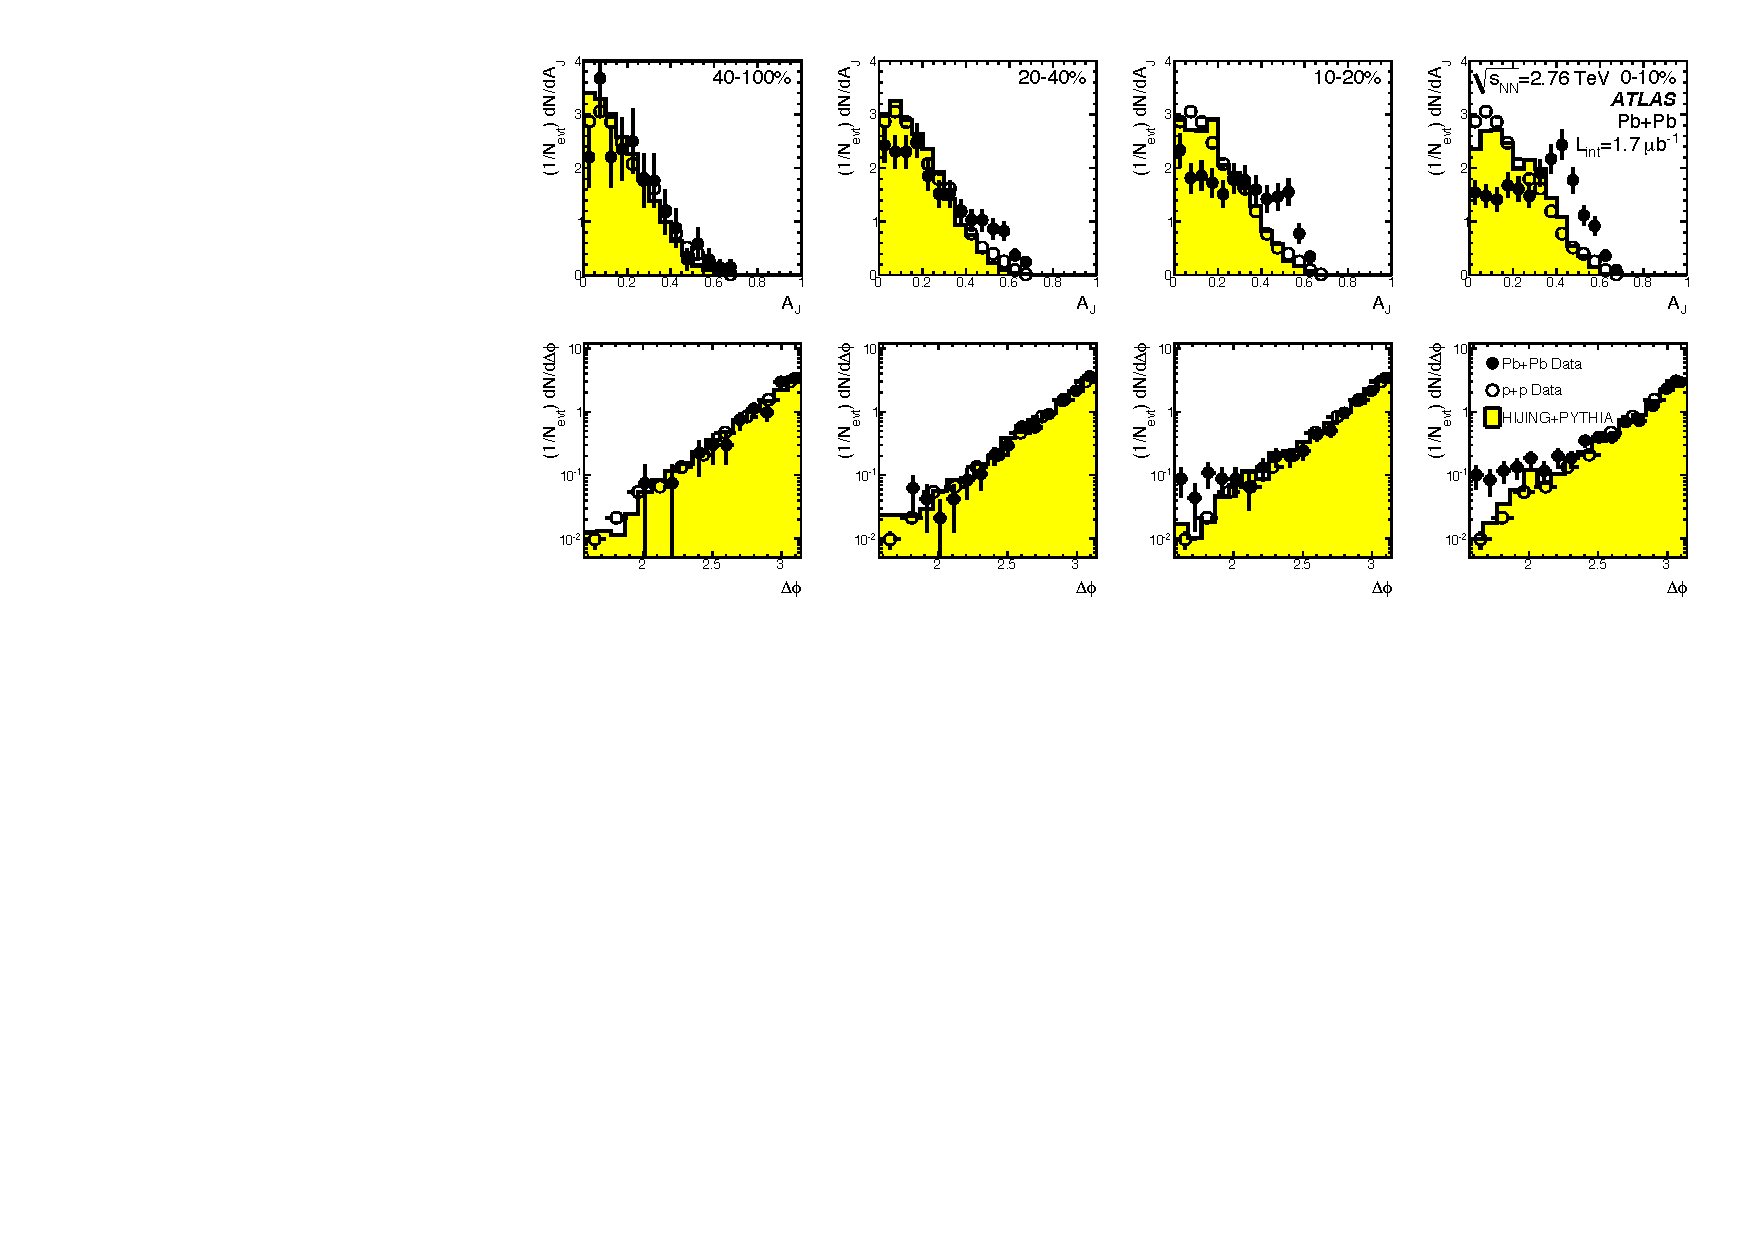
\includegraphics[width=0.8\textwidth]{jetfigures/final_4x2_23_newpp.pdf}
\caption{
(top) Dijet asymmetry distributions for data (points) and {\sc{hijing+pythia}} 
simulations (solid yellow histograms), as a function of collision centrality.  
Proton-proton data from $\sqrt{s}=7$\TeV\ is shown as open circles.
(bottom) Distribution of $\dphi$ between the two jets, 
for data and {\sc{hijing+pythia}}, shown in four bins of centrality.
Reproduced from~\cite{Aad:2010bu}.}
\label{fig:GR:final_4x2}
\end{center}
\end{figure}

A clear centrality evolution of the dijet asymmetry distribution can be seen, while the azimuthal
dijet correlations remain largely unchanged. For peripheral events, the \PbPb\ dijet asymmetry
is comparable to that seen in PYTHIA and \pp\ collisions. For central events however,
the $A_J$ distribution widens significantly, showing a large increase in unbalanced
dijet events. 
A similar measurement by CMS, using the full 2010 \PbPb\ data set, confirmed these 
observations~\cite{Chatrchyan:2011sx}.
The observed trend can be naturally understood in models of parton energy
loss in the hot and dense medium, where the back-to-back partons will typically traverse
different path lengths, and therefore suffer different amounts of energy loss. 

The initial ATLAS and CMS dijet asymmetry analyses were extended using a 
large dataset of \PbPb\ collisions
collected in 2011 by the CMS collaboration at $\rootsNN=2.76$\TeV~\cite{CMS_dijet}. For this analysis, the events were 
reconstructed using the  CMS ``particle-flow" algorithm~\cite{CMS-PAS-PFT-10-002,MattPFlow}, 
which attempts to identify all stable particles in an
event (electrons, muons, photons, charged and neutral hadrons)
by combining information from all sub-detector systems.
Jets were then reconstructed, after background subtraction, using the anti-$k_T$ algorithm 
with radius parameter R = 0.3~\cite{Cacciari:2008gp}.

Figure~\ref{fig:GR:CMS_dijet_pt} presents the dijet asymmetry in bins of leading jet
\pT, for 0--20\% central events, allowing a study the momentum dependence of the amount of energy loss.
The distributions show the \ptrat\ ratio, instead of $A_j$,  as a more intuitive
way of quantifying the dijet momentum asymmetry. The data are compared to \PYTHYD\ simulations, where
(unquenched) PYTHIA dijet events are embedded into HYDJET background events, and 
HYDJET is tuned to reproduce multiplicity, \pT\ spectra and elliptic flow of \PbPb\ data events.

\begin{figure}[!th]
\begin{center}
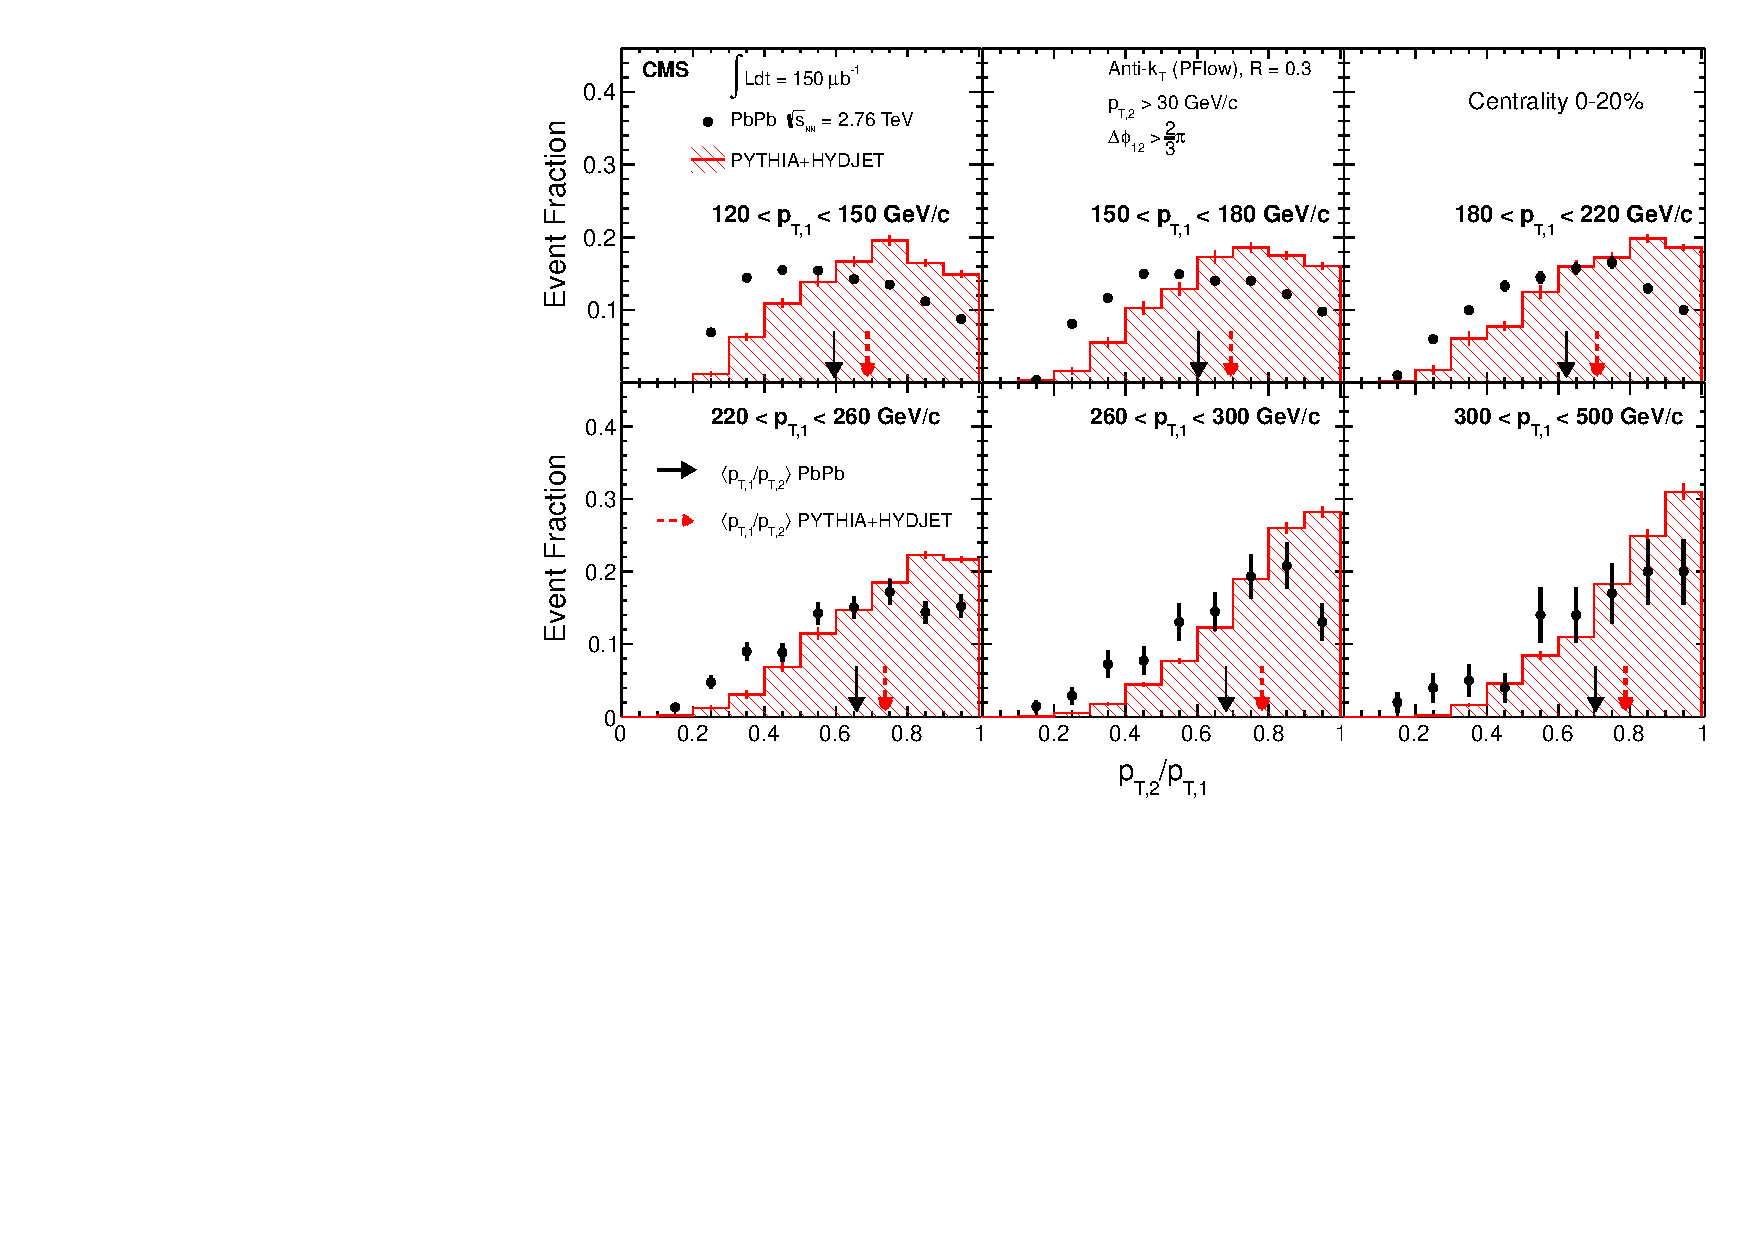
\includegraphics[width=0.6\textwidth]{jetfigures/dijet_imbalance5_0to20_pt_20120103_subt.pdf}
\caption{Dijet asymmetry ratio, $A_{J}$, in bins of leading jet transverse momentum from
120 $ < \ptlead < 150$~GeV/c to $\ptlead > 300$~GeV/c for
  subleading jets of $\ptsub> 30$~GeV/c
and $\dphi>2\pi/3$ between leading and subleading jets.
Results for 0--20\% central \PbPb\ events are shown as points, while the histogram
shows the results for
PYTHIA dijets embedded into HYDJET \PbPb\ simulated events. The error bars represent the statistical uncertainties.
Reproduced from~\cite{CMS_dijet}.}
\label{fig:GR:CMS_dijet_pt}
\end{center}
\end{figure}
One observes a strong evolution in the shape of the distribution across the
various \pT\ bins. However, a significant difference between \PbPb\ data and
\PYTHYD\ simulations persists even for the highest \pT\ bin.
The jet momentum dependence of the energy loss can then be examined by measuring the
average dijet asymmetry as a function of leading jet momentum. This was studied by CMS,
using $\langle \ptsub/\ptlead \rangle$. Figure~\ref{fig:GR:CMS_pt_ratio}
shows the \pT\ dependence of this ratio for three
bins of collision centrality, with \PYTHYD\ simulations shown
as squares and \PbPb\ data shown as points.

\begin{figure}[!th]
\begin{center}
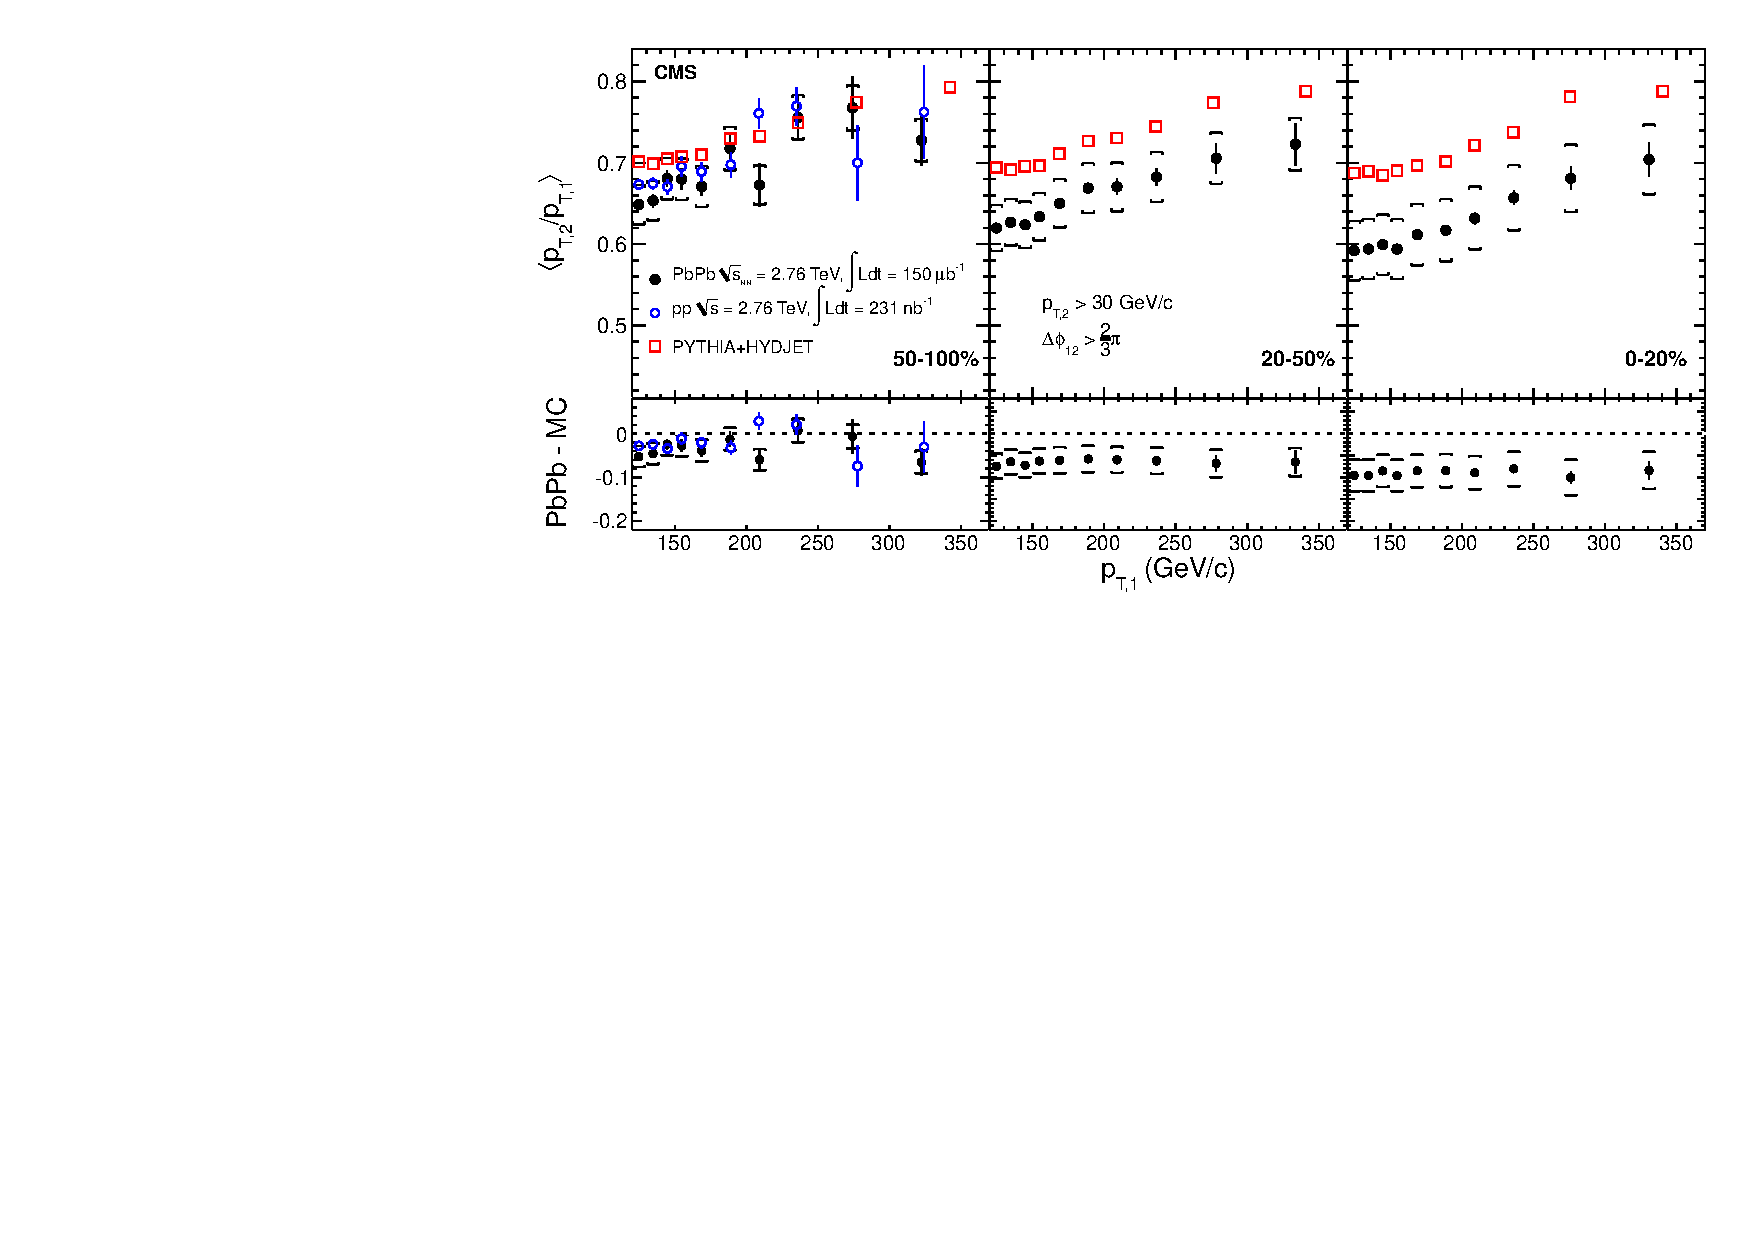
\includegraphics[width=0.6\textwidth]{jetfigures/deltaPtOverPt5_lead120_sub30_diff_20120103.pdf}
\caption{(Top): Dijet momentum ratio $\langle \ptsub/\ptlead \rangle$ as a function of
leading jet \pT\ in three bins of collision centrality.
\PbPb\ data are shown as points, with brackets indicating systematic uncertainties.  
\PYTHYD\ calculations are shown as squares. In the peripheral bin,
\pp\ data are displayed as open circles.
(Bottom): Difference of $\langle \ptsub/\ptlead \rangle$ between the \PbPb\ results and \PYTHYD\ reference.
Reproduced from~\cite{CMS_dijet}.}
\label{fig:GR:CMS_pt_ratio}
\end{center}
\end{figure}

For all data and simulations, a rising trend of $\langle \ptsub/\ptlead \rangle$ as a function
of leading jet momentum is seen. This is a result of the improving jet energy resolution
with increasing jet \pT\ and the evolution in jet kinematics, which is described by the PYTHIA
calculations. Importantly, the data show a significantly larger jet asymmetry in central events
than in the simulations and in peripheral and \pp\ data. This effect persists to the
highest \pT\ measured, showing that even the highest \pT\ jets in \PbPb\ collisions ($\pT > 350$\GeVc)
suffer energy loss as they traverse the medium. A detailed understanding of the energy loss
\pT\ dependence (e.g.\ fractional vs constant energy loss) will require a full jet MC calculation
taking the detector response as a function of \pT\ into account.

\subsection{Suppression of jet yields}

A complementary approach to the study of parton energy loss using dijet asymmetry measurements
is offered by studies of the nuclear modification factor \Raa\ of jet yields relative
to a \pp\ reference or the centrality evolution of \Rcp\ relative to peripheral events.

Measurements of the inclusive jet production rates were performed by ATLAS~\cite{Aad:2012is} and 
ALICE~\cite{Abelev:2013kqa}.
As a result of the path length dependence of parton energy loss in the medium, 
a reduction in the observed jet yield at a given \pT\ is expected for more 
central \PbPb\ collisions, compared to an \Ncoll\ scaled \pp\ or peripheral reference.

\begin{figure}[!th]
\begin{center}
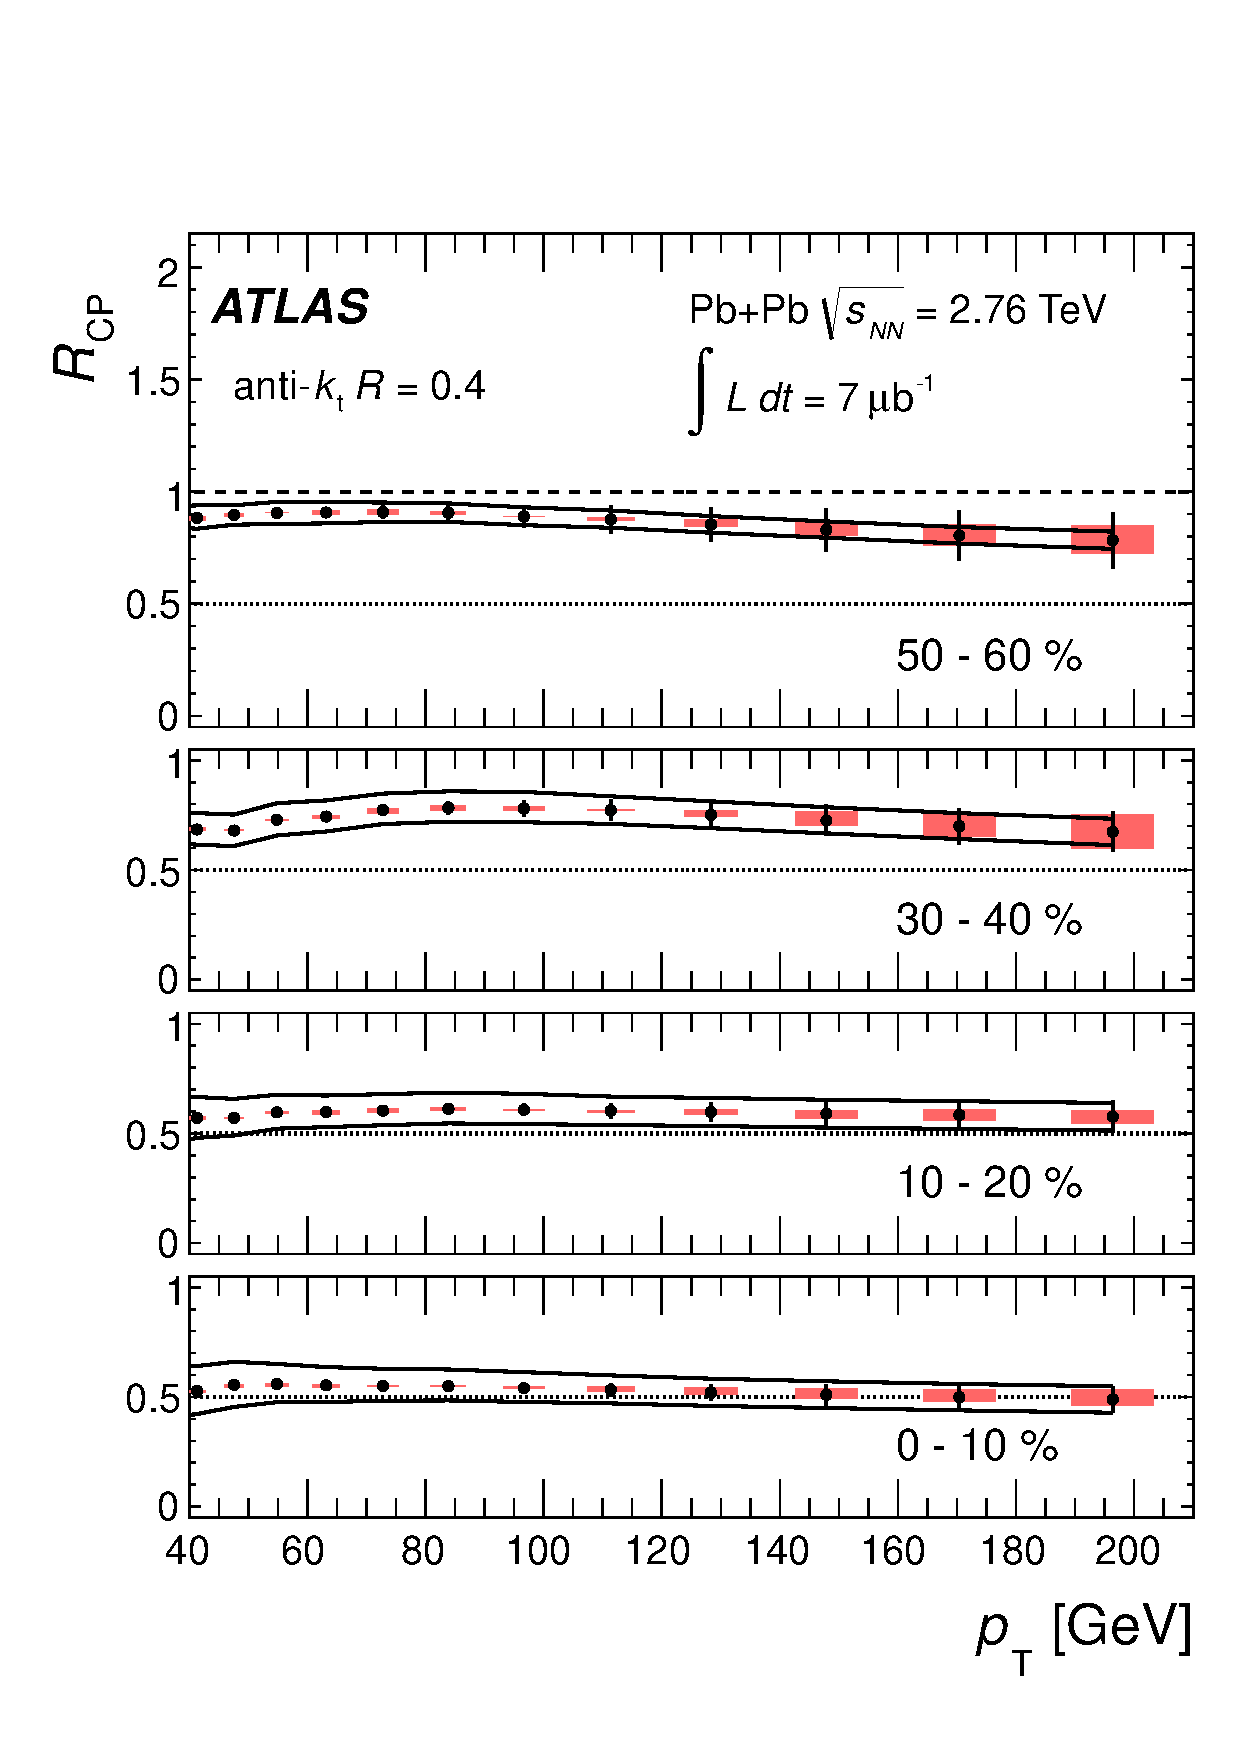
\includegraphics[width=0.49\textwidth]{jetfigures/ATLAS_jetRCP_04.pdf}
\caption{
\pT\ dependence of jet \Rcp\ for  $R=0.4$ jets,
in four bins of collision centrality. Error bars indicate
statistical errors while shaded boxes indicate
partially correlated systematic uncertainties. 
The solid lines show fully correlated uncertainties. Reproduced from~\cite{Aad:2012is}.}
\label{fig:GR:rcprfour}
\end{center}
\end{figure}
The resulting \Rcp\ values are shown in Figure~\ref{fig:GR:rcprfour}
for  \RFour\ jets as a function of jet \pT\ in four bins
of collision centrality.
Uncertainties are shown as statistical uncertainties, partially correlated systematic
uncertainties, and fully correlated uncertainties.

For all centralities only a weak dependence of \Rcp\ on jet \pT\ is observed.
In contrast, a strong suppression of the jet yield is evident in
central collisions, with \Rcp\ only reaching a value of about 0.5.
This is reminiscent of the value of charged hadron \Raa\ observed
by CMS at very high \pT\, which also reaches a value of about 0.5.
The centrality evolution of \Rcp\ is consistent with expectations
based on the increasing in-medium pathlength traversed by the partons.

Further insight into the pathlenth dependence of parton energy
loss may be gained by studying the dependence of the jet yield
on the jets azimuthal angle relative to the event plane
in peripheral \PbPb\ collisions. This allows the selection of jets
traversing different length of the medium at the same medium
conditions, whereas the centrality dependence of \Rcp\ reflects
both the changing pathlength and potential changes in the medium
density with centrality.

Related measurements have been performed using the azimuthal dependence
of charged hadron yields at intermediate \pT\
\cite{Adams:2004wz,Adler:2006bw,Adare:2010sp, ATLAS:2011ah, Abelev:2012di}.
and very high \pT \cite{Chatrchyan:2012xq}. For mid-peripheral events,
a finite \vtwo\ for charged hadrons was observed for \pT\ in excess of 40\GeVc.
Compared to these results, jet based measurements offer the advantage
of a more direct relationship between \pT\ and direction of the observed
jet and the initial parton.

\begin{figure}[!th]
\begin{center}
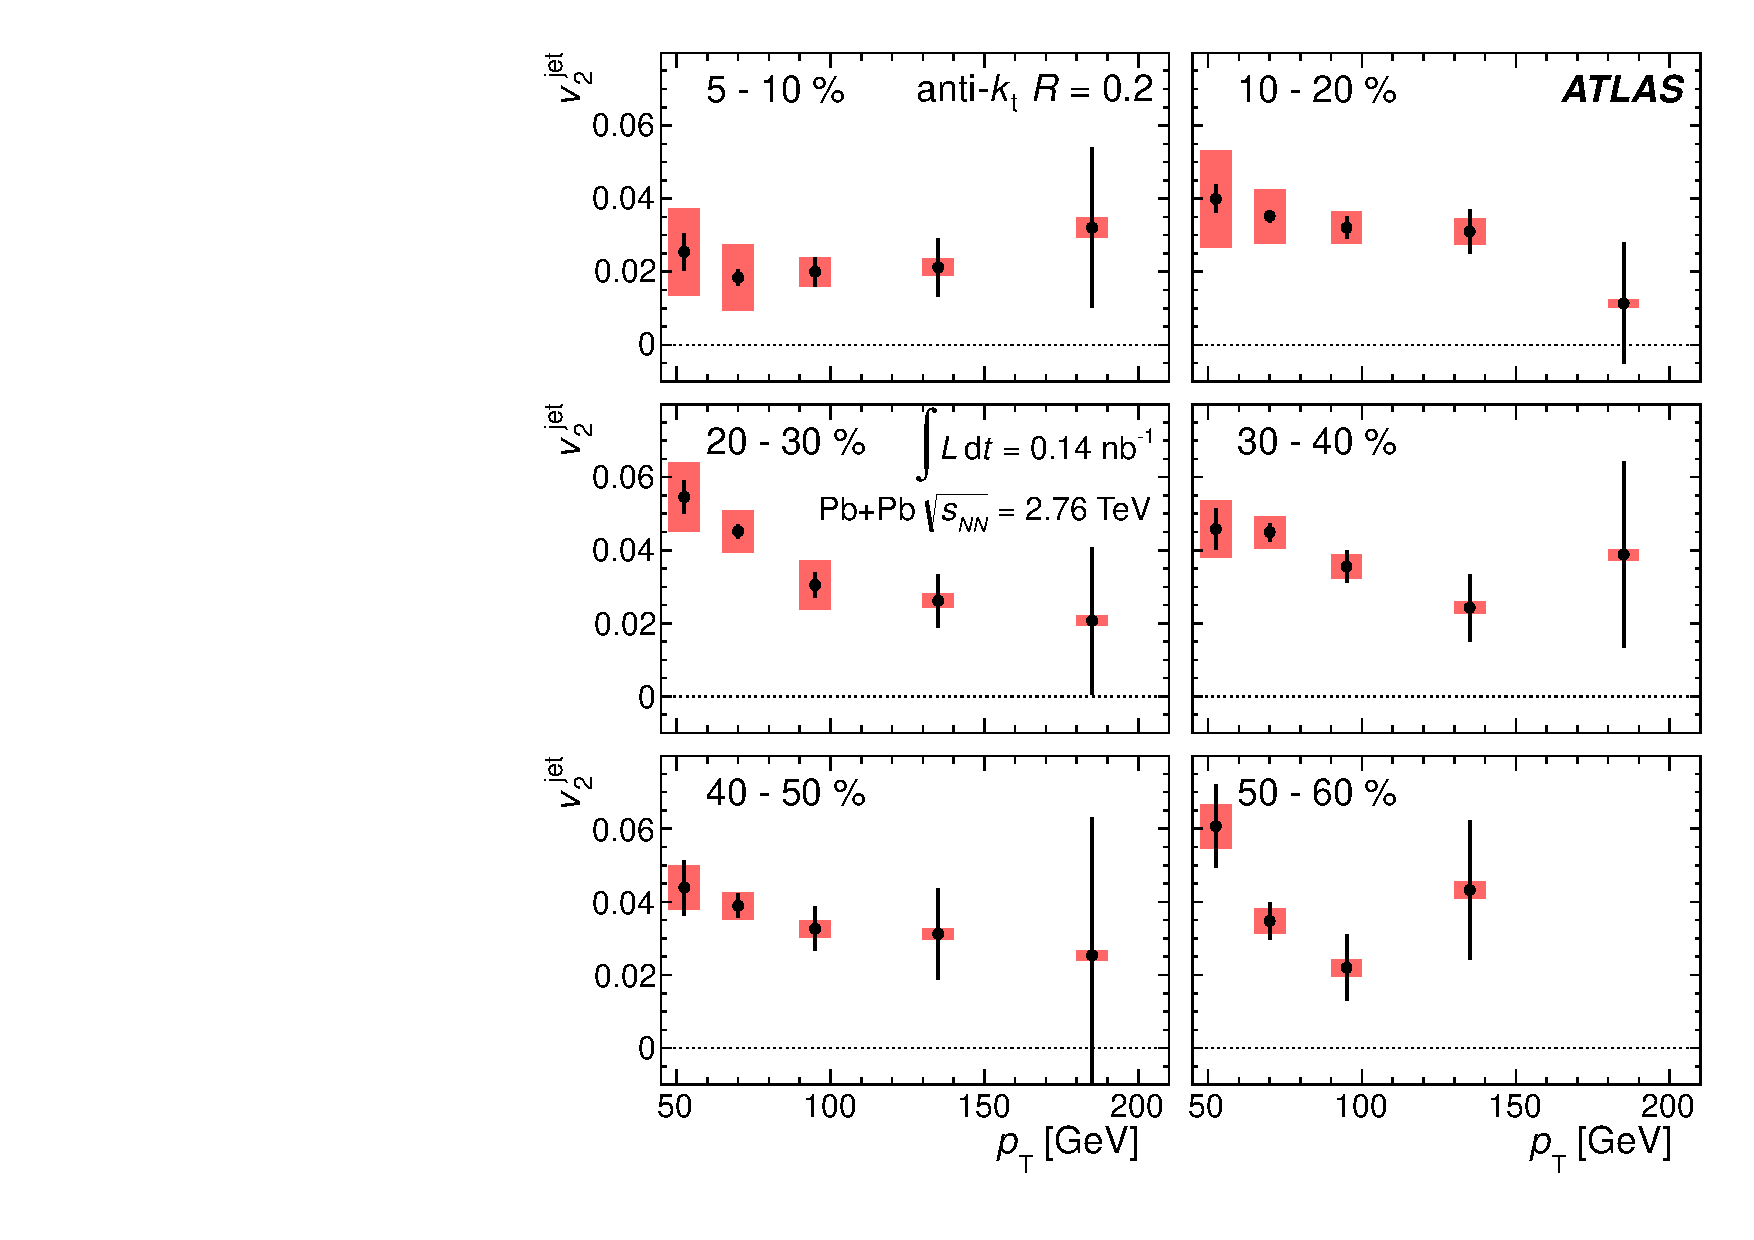
\includegraphics[width=0.49\textwidth]{jetfigures/ATLAS_jetv2.pdf}
\caption{\vtjet\ as a function of jet \pT\ in six bins of 
collision centrality.
Error bars indicate statistical uncertainties and 
systematic uncertainties are shown as shaded boxes. Reproduced from~\cite{Aad:2013sla}}
\label{fig:GR:ATLAS_jet_v2}
\end{center}
\end{figure}

The result of the ATLAS \vtwo\ measurement for jets reconstructed with the anti-$k_T$
algorithm in 2.76\TeV\ \PbPb\ collisions is shown in Fig.~\ref{fig:GR:ATLAS_jet_v2}
as a function of jet \pT\ in bins of collision centrality~\cite{Aad:2013sla}. A finite
value of \vtwo\ is observed for all centrality and \pT, reaching up to 0.05 for
mid-central collisions and low jet \pT. The results are in good agreement
with those for high \pT\ charged hadrons covering a comparable range
of initial parton \pT~\cite{Chatrchyan:2012xq}.

\subsection{Modification of jet structure}

In addition to the \pT\ and centrality dependence of the suppression, its dependence on the 
jet clustering radius parameter or cone-size is also of great interest, as different energy loss 
mechanisms may lead to different amounts of energy transport out of the jet cone
\cite{Vitev:2008rz, Vitev:2009rd,He:2011pd}. This should manifest as a cone-size
dependence of the observed jet suppression.
\begin{figure}[!th]
\begin{center}
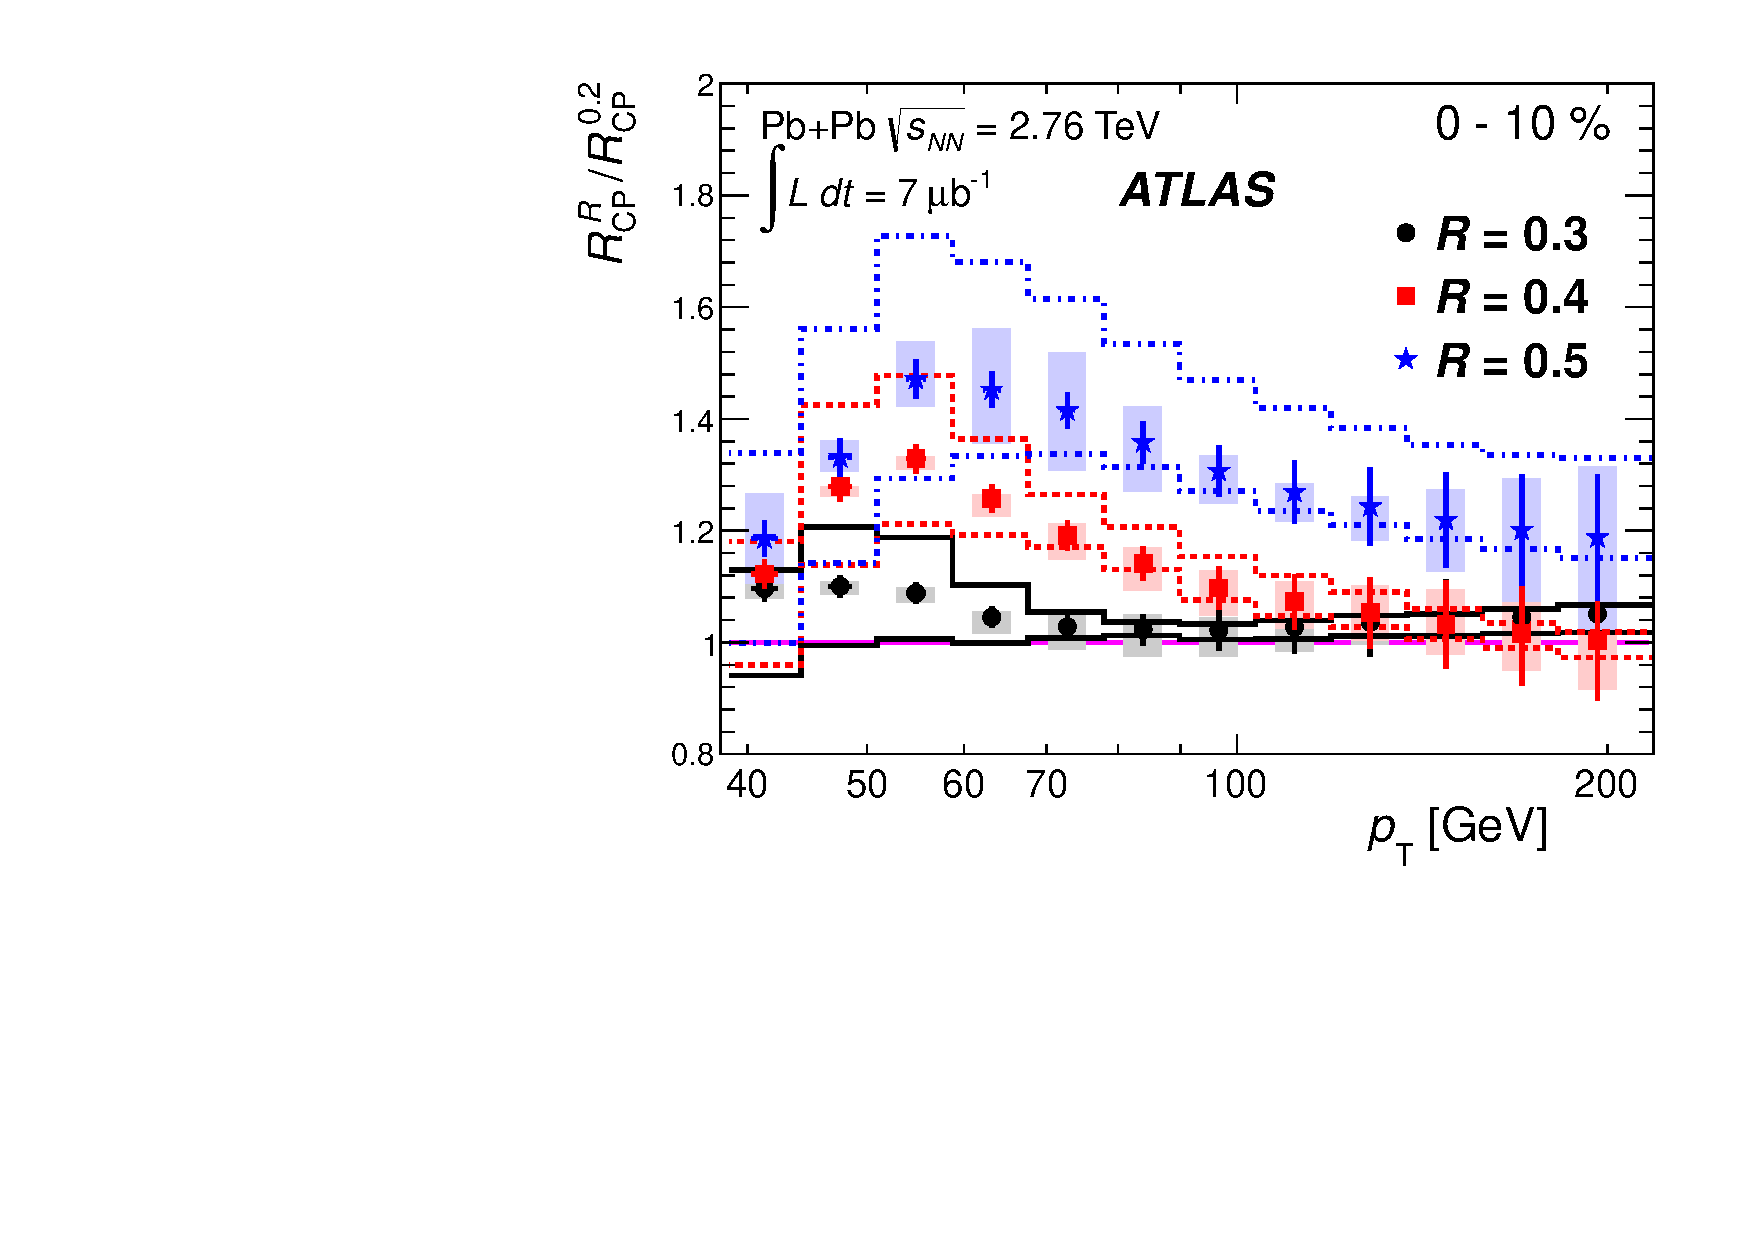
\includegraphics[width=0.49\textwidth]{jetfigures/ATLAS_jetRCP_size.pdf}
\caption{
Ratios of \Rcp\ values between $R = 0.3, 0.4$ and 0.5 jets and $R =
0.2$ jets as a function of \pT\ in the 0--10\% centrality bin. The
error bars show statistical uncertainties. The shaded boxes
indicate partially correlated systematic errors. The lines indicate
systematic errors that are fully correlated between different \pT\ bins.
Reproduced from~\cite{Aad:2012is}.
}
\label{fig:GR:ATLAS_jetRCP_size}
\end{center}
\end{figure}

Such a dependence can be seen in Fig.\ref{fig:GR:ATLAS_jetRCP_size}, which
shows the ratio of \Rcp\ values for $R = 0.3, 0.4$ and 0.5 jets compared
to an $R = 0.2$ jets baseline, as a function of \pT\ for central events,
measured by ATLAS~\cite{Aad:2012is}.

The cancellation of various systematic uncertainties allows the observation of a
significant jet radius dependence of \Rcp, in particular for
lower jet \pT. A detailed comparison needs to consider the \pT\ associated with
using different radius parameters to reconstruct the same jets.

Further insight into modifications of the momentum and angular structure
of jets in heavy-ion collisions can be gained by measurements of
observables used for jet studies in elementary interactions, such as
fragmentation functions and jet shapes.
Fragmentation functions describe the probability for a parton to fragment into
hadrons carrying certain fractions of the parton energy.
In vacuum, the parton radiation and splitting processes lead to a
well-understood characteristic shape of the fragmentation function \cite{Dokshitzer:1991wu}.

\begin{figure}[!ht]
\begin{center}
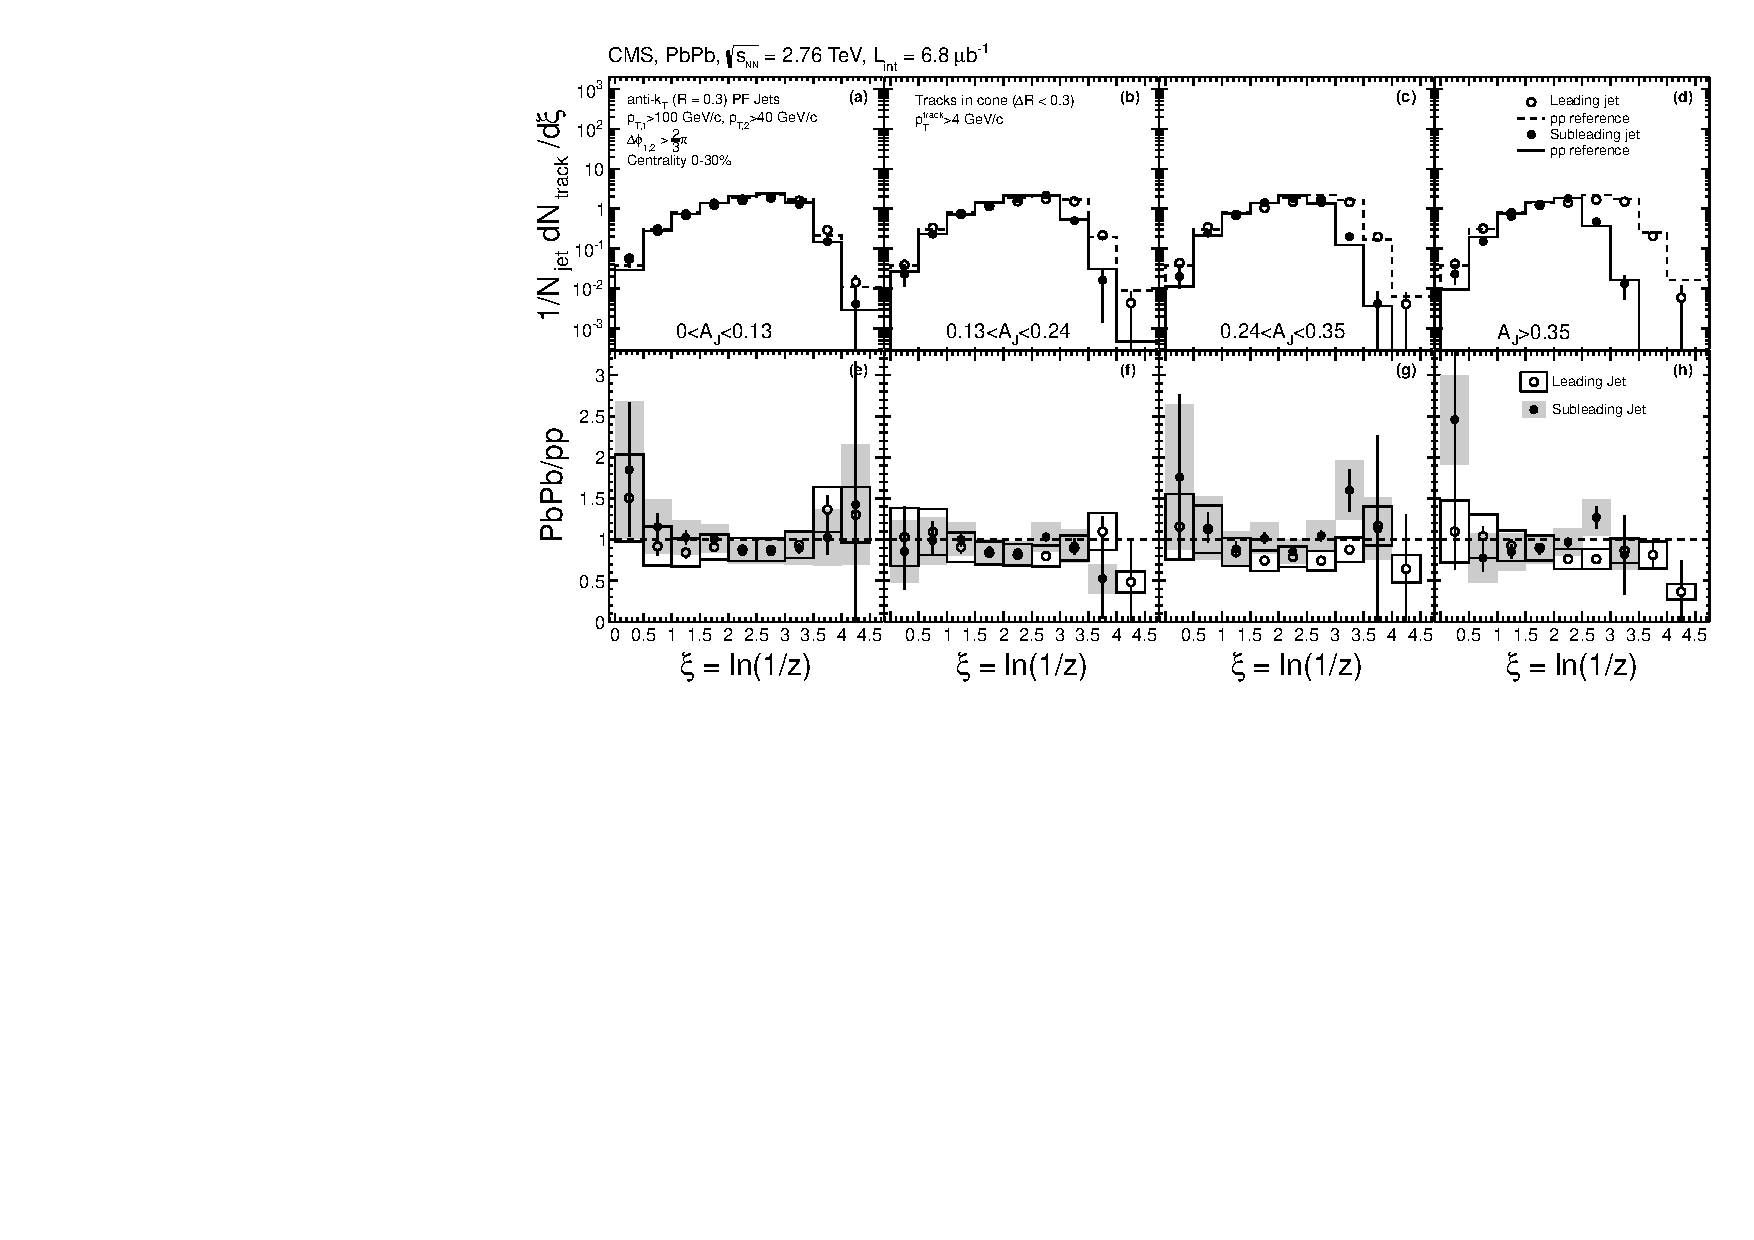
\includegraphics[width=0.8\textwidth]{jetfigures/xsi_div_both_effv9_l100s40_0to12_dphi20eta20dr3pt4id1_cwt_ppDiv_gray.pdf}
\caption{Top row: Fragmentation functions for the leading (open circles) and subleading (solid points) 
jets in four regions of $\AJ$ in central \PbPb\ collisions compared to the \pp\ reference.
Bottom row: Ratio of each fragmentation function to its \pp-based reference.
Error bars shown are statistical. The systematic uncertainty is
represented by open boxes (leading jet) or gray boxes (subleading jet).
Reproduced from~\cite{Chatrchyan:2012gw}.
}

\label{fig:GR:CMS_jetFF}
\end{center}
\end{figure}
Figure~\ref{fig:GR:CMS_jetFF} shows the fragmentation functions 
for leading and subleading jets for 0-30\% central collisions, obtained
by CMS~\cite{Chatrchyan:2012gw}. Data for \PbPb\ are shown in 
bins of dijet asymmetry $A_J$, and compared to a \pp\ based reference.
The lower row of plots shows the ratios between the \PbPb\
and \pp-based fragmentation functions. It is important to note, and has 
led to occasional confusion, that these fragmentation functions are 
measured relative to the \em observed \em jet momentum, not with respect
to the initial parent parton momentum, which can not be directly observed
for dijet events in hadronic collisions.
Energy radiated outside of the jet cone, or at \pT\ of less than $\approx 1$\GeVc\
is not included in the jet energy determination.

Within the uncertainties of this first measurement, no significant modification of
the fragmentation functions in \PbPb\ collisions is observed. This is true even for
dijets with large asymmetry, i.e.\ where the subleading jet has suffered significant
energy loss. It is important to note however that only hadron fragments with $\pT > 4$\GeVc
have been considered in this measurement. i


Complementary information about the angular structure of the jets and its modification
by the in-medium shower evolution can be obtained by measuring jet shapes, i.e.\ the
jet transverse momentum profile as a function of radial distance to the jet axis
\cite{MehtarTani:2010ma,Idilbi:2008vm,CasalderreySolana:2011rz,CasalderreySolana:2011rq,Neufeld:2011yh,Blaizot:2012fh,Fickinger:2013xwa}.
The differential jet shape, $\rho(r)$, is defined as
\begin{equation}
\rho(r) = \frac{1}{\delta r} \frac{1}{N_{\mbox{jet}}} \sum_{\mbox{jets}}
\frac{\sum\limits_{{r - \delta r/2}}^{{r + \delta r/2}}{\pT^{\mbox{track}}}}{\pT^{\mbox{jet}}}
\label{eq:rho(r)}
\end{equation}
Here $r$ is the radial distance from the jet axis
and the transverse momenta of the reconstructed track and jet are
$\pT^{\mbox{jet}}$ and $\pT^{\mbox{track}}$, respectively.

In the CMS measurement of jet shapes\cite{Chatrchyan:2013kwa}, the jet cone is divided into six concentric rings
with radial width $\delta r = 0.05$. The transverse momentum profile is determined using
the \pT\ sum for charged particles with $\pT > 1\GeVc$ in each ring, compared to
the fraction of the total jet \pT\ carried by these particles. As for the fragmentation
functions, the \PbPb\ jet shapes are compared to a \pp\ based reference.

\begin{figure}[!ht]
\begin{center}
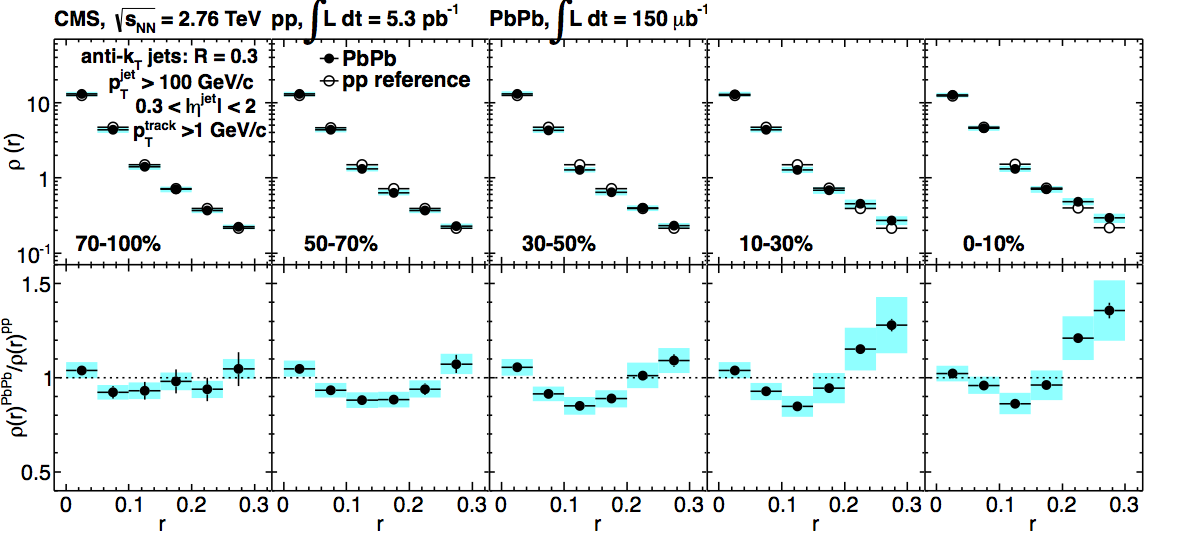
\includegraphics[width=0.98\textwidth]{jetfigures/JetShapes_GR.png}
\caption{\label{fig:JSRatio}
(Top): Differential jet shapes in \PbPb\ collisions (filled circles)
as a function of distance from the jet axis for inclusive jets with $\pT^{\mbox{jet}} >100\GeVc$
in five bins of centrality.  The \pp-based reference is shown with open symbols.
The shaded regions represent the \PbPb\ systematic uncertainties.
Statistical uncertainties are smaller than the marker size.
(Bottom): Jet shape ratios $\rho(r)^{\PbPb}/\rho(r)^{\pp}$.
Error bars show the statistical uncertainties and shaded boxes indicate the systematic uncertainties. 
Reproduced from~\cite{Chatrchyan:2013kwa}}
\label{fig:GR:CMS_jetshapes}
\end{center}
\end{figure}

The top row of Fig.~\ref{fig:GR:CMS_jetshapes} shows the differential jet shapes measured in \PbPb\
collisions and the \pp\ based reference, while the bottom row shows the ratio of the \PbPb\ and \pp\
distributions. The results are presented in five bins of collision centrality, from
most peripheral 70--100\% (left) to most central 0--10\% (right). For
both systems, only a small amount of the total jet energy
is carried by particles more than  $r> 0.2$ away from the jet axis. However, for central
\PbPb\ collisions a large enhancement of the energy fraction at the largest distance
to the jet axis ($r = $0.25-0.3) can be seen.
This is qualitatively consistent with the \Rcp\ ratios for different jet radii seen by ATLAS,
where also an additional part of the jet energy is captured when moving beyond $R = 0.2$.
This observation is in line with the trends predicted in
\cite{Vitev:2008rz,Renk:2009hv}, although these calculations were
done for a different energy and and at parton level rather than hadron level.

\subsection{Energy flow in dijet events}

The jet measurements discussed so far clearly demonstrate that partons traversing the hot and dense
medium suffer significant path-length dependent energy loss. A fraction of the ``lost'' energy
can be recovered at radii of $r=$0.2-0.5 from the jet axis, although even for the largest radius
parameters used at LHC, a large suppression of inclusive jets and large dijet asymmetries are
observed.

This naturally begs the question of the detailed energy flow in the events containing asymmetric
dijets events, i.e.\ what is the angular and momentum distribution of the particles carrying
the complementary momentum balance to the asymmetric dijet system? A priori the energy balance
could possibly be found at low (thermal) momenta and very large radial distance to the jet axis.
Therefore traditional jet-track correlation techniques relying on background subtraction are ill suited
to answer this question. Even the largest dijet energy differences of several 10's of \GeV\
correspond to only a per-mille fraction of the total transverse energy carried by the underlying 
event. The presence of long-range flow correlations, and biases in event properties when requiring 
high-\pT\ dijets, have made a sufficiently precise description of the underlying event using e.g.\ 
mixed events intractable so far.

Information about the overall momentum balance in the dijet events can be obtained by exploiting
conservation of transverse momentum. CMS studied the transverse momentum balance in these events
using the projection of missing \pT\ of reconstructed charged tracks onto the leading 
jet axis~\cite{Chatrchyan:2011sx}. 
Event-by-event, this was calculated as 
\begin{equation}
\displaystyle{\not} p_{\mathrm{T}}^{\parallel} =
\sum_{\rm i}{ -p_{\mathrm{T}}^{\rm i}\cos{(\varphi_{\rm i}-\varphi_{\rm Leading\ Jet})}},
\end{equation}
summing all tracks with $\pT > 0.5$~\GeVc\ and $|\eta| < 2.4$.
Leading and subleading jets were required to have $|\eta| < 1.6$.
Instead of a background subtraction, this method relies on the cancellation of the
underlying event fluctuations when averaging over many events to obtain
$\langle \displaystyle{\not} p_{\mathrm{T}}^{\parallel} \rangle$.

Figure~\ref{fig:GR:CMS_missingpT} shows $\langle \displaystyle{\not} p_{\mathrm{T}}^{\parallel} \rangle$
as a function of \AJ\ for two angular regions relative to the leading and subleading
jet axes, ``in-cone'' ($\Delta R < 0.8$) and ``out-of-cone'' ($\Delta R > 0.8$).
This measurement requires a tight $\dphi > 5 \pi/6$ selection for the dijet, to ensure that the 
leading and subleading cones sample equivalent regions of the underlying event background on average. 
The top row shows results for  {\sc{pythia+hydjet}} simulations and the bottom row shows
\PbPb\ data. Integrating over all particle momentum ranges (solid points),
 the overall momentum balance of the events is recovered within uncertainties
as the negative $\langle \displaystyle{\not} p_{\mathrm{T}}^{\parallel} \rangle$ in
the in-cone region is balanced by a positive value in the out-of-cone angular range.

\begin{figure}[!ht]
\begin{center}
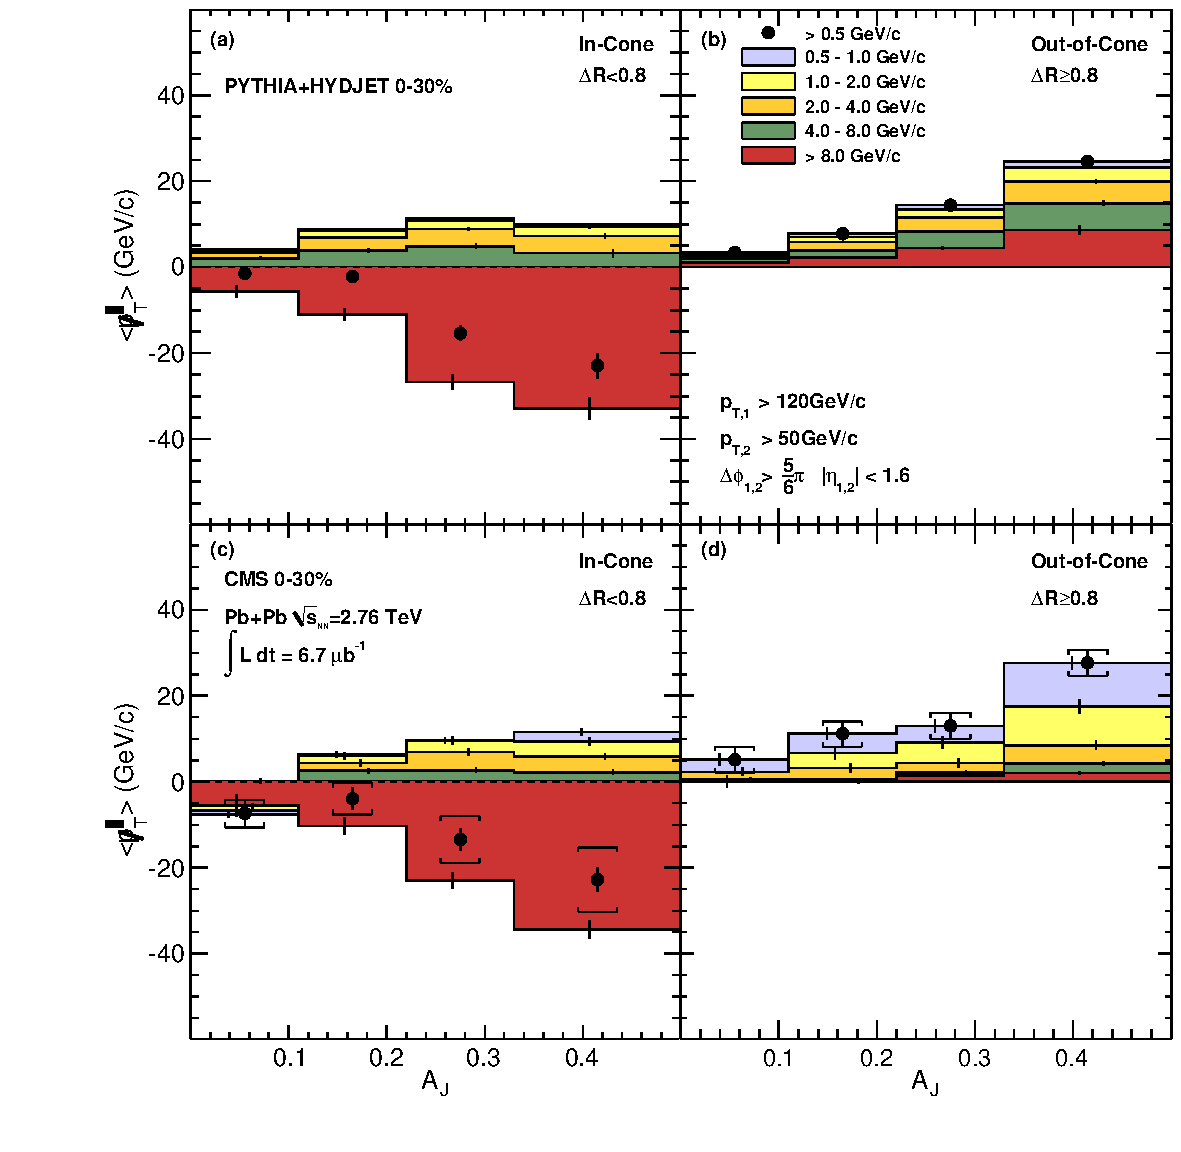
\includegraphics[width=0.7\textwidth]{jetfigures/missingPtParallel-Corrected-data-InConeOutConeDPhiCut_ntv6_2.pdf}
\caption{Average missing transverse momentum,
$\langle \displaystyle{\not} p_{\mathrm{T}}^{\parallel} \rangle$,
for tracks with $\pT > 0.5$\GeVc, projected onto the leading jet axis (solid circles).
The $\langle \displaystyle{\not} p_{\mathrm{T}}^{\parallel} \rangle$ values are
shown as a function of dijet asymmetry
$A_J$ for 0--30\% centrality, inside ($\Delta R < 0.8$) one of the leading or subleading jet cones (left) and
outside ($\Delta R > 0.8$) the leading and subleading jet cones (right).
For the solid circles, vertical bars and brackets represent
the statistical and systematic uncertainties, respectively.
For the individual $\pT$ ranges, the statistical uncertainties are shown as vertical bars.
Reproduced from~\cite{Chatrchyan:2011sx}.}
\label{fig:GR:CMS_missingpT}
\end{center}
\end{figure}

Focussing on asymmetric dijet events ($\AJ > 0.33$), both data and MC exhibit an
 in-cone imbalance of $\langle \displaystyle{\not} p_{\mathrm{T}}^{\parallel} \rangle \approx
-20$~\GeVc. This is balanced by an out-of-cone contribution of
$\langle \displaystyle{\not} p_{\mathrm{T}}^{\parallel} \rangle \approx 20$~\GeVc. The key
observation is that in the \PbPb\ data the out-of-cone contribution is found in the $0.5 < \pT < 4$~\GeVc\ region,
while in MC more than 50\% of the balance is carried at high $\pT > 4$~\GeVc. The MC
results can be interpreted as resulting from initial or final-state radiation (e.g.\ three-jet events).
For \PbPb\ events with large \AJ\ a large part of the momentum balance is
carried by soft particles ($\pT < 2$~\GeVc) at large angles to the jet axes ($\Delta R > 0.8$). This measurement
therefore has provided crucial information about the fundamental properties of the energy loss process
in the medium.

\subsection{Photon-jet correlations}

The use of the dijet and inclusive jet observables discussed in the previous sections
to extract information
about the absolute energy loss of the partons traversing the medium suffers from
uncertainties about the initial parton kinematics. E.g.\ for the dijet asymmetry
measurements in general both partons will suffer some amount of path-length dependent
energy loss, leading to ambiguities in the quantitative interpretation of the results
due to possible surface-biases.

These ambiguities can be largely overcome in studies of photon-jet events,
where the photon closely determines both the initial direction and momentum
of the back-to-back associated parton on an event-by-event basis~\cite{Wang:1996yh}.
Events where the photon and parton initial kinematics are most closely correlated
can be selected experimentally using an isolation requirement, which
increases the fraction of events with ``leading order'' prompt photons in
the photon-jet sample. The first measurement of isolated photon-jet correlations
was performed by CMS for a 150\mubinv \PbPb\ dataset~\cite{Chatrchyan:2012gt}.
To select ``isolated photons'', the energy in a cone around 
the photon candidate was required to be less than a threshold parameter~\cite{HIPhoton},
following a standard procedure developed for the analysis of \pp\ collisions. In the \PbPb\ 
environment, the isolation cut is applied after a subtraction of an event-by-event 
estimate of the underlying event contribution.

Following the approach for the study of dijet correlations, the photon-jet pairs
are characterized in terms of their azimuthal correlation, $\dphijg = |\phij - \phig|$,
 and momentum ratio, $\xjg = \ptj/\ptg$. In addition, the fraction of photons without
back-to-back jet partner,  \rjg, is studied, to provide information about
events where the jet lost sufficient energy to fall below the detection threshold.
For the CMS photon-jet analysis, photons were required to have $\ptg > 60\GeVc$
and  $|\eta^\gamma|<1.44$. The associated jets were selected with
$\ptj > 30\GeVc$ and $|\eta^{\mbox{Jet}}|<1.6$. To study the correlations of
photons with their associated jets (rather than photon-inclusive jet or photon-leading
jet correlations), contributions from
coincidental photon-jet pairs were removed using a mixed event technique. In
addition, the contribution of background photons from e.g.\ hadron decays
were corrected using a data driven technique. The purity of the isolated photon-jet
sample was further enhanced by requiring $\dphijg > \frac{7}{8}\pi$.
Similar to the dijet correlations, no angular broadening
beyond the \pp\ data and MC reference was seen in the \PbPb\ data.

The photon-jet momentum correlations in \PbPb\ data were compared to a \PYTHYD\ reference
calculation as a function of collision centrality. The resulting
\xjg\ distributions are shown in Fig.~\ref{fig:GR:InclPtRatio_qcdPhoRef_pp2760-xJ30G60}.
Also shown is \avexjg\ distribution for 2.76\TeV\ \pp\ data, showing consistency
with the \PYTHYD\ calculation within the large statistical uncertainties.
The separate open and shaded red systematic uncertainty boxes illustrate the
anti-correlation of uncertainties across bins for the unity-normalized distributions.

\begin{figure}[!ht]
\begin{center}
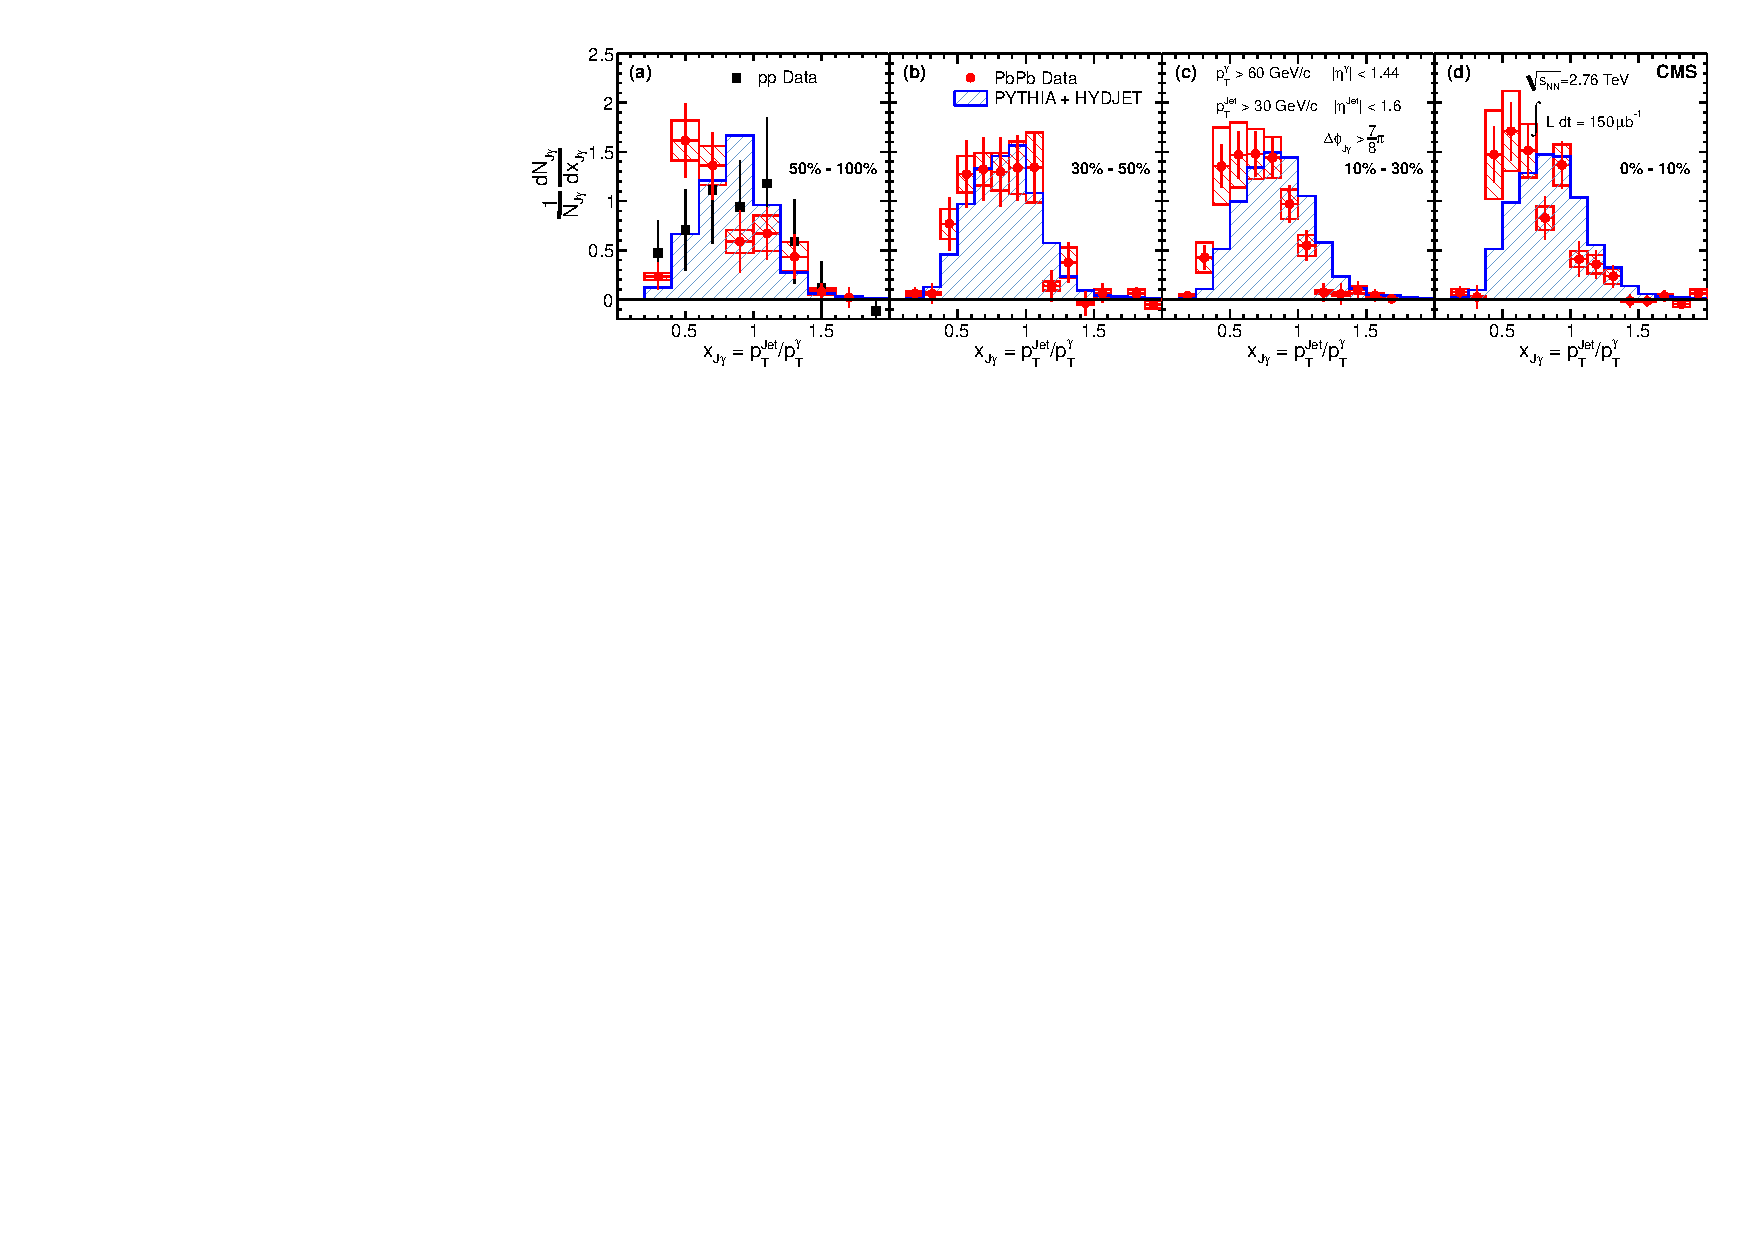
\includegraphics[width=0.98\textwidth]{jetfigures/Photonv7_Paper_InclPtRatio_all_cent4_G60J30_subDPhi1SS1_Isol0_Norm1log1.pdf}
\caption[]{\label{fig:GR:InclPtRatio_qcdPhoRef_pp2760-xJ30G60} Distribution of the photon/jet 
momentum ratio, \xjg, in four bins of collision centrality. 
  The distributions are normalised to unit area. All panels compare
\PbPb\ data (filled circles) to \pp\ data at
  2.76\TeV\ (filled squares), and to the \PYTHYD\ MC simulations
  (shaded histogram). Error bars show the statistical uncertainties and
boxes show the (anti-correlated) systematic uncertainties. Reproduced from~\cite{Chatrchyan:2012gt}.}
\label{fig:GR:CMS_xjg}
\end{center}
\end{figure}

For the most central events, the  photon-jet momentum balance  was found to be
$\avexjg_{0-10\%} = 0.73 \pm 0.02 \mbox{(stat.)} \pm 0.04 \mbox{(syst.)}$, compared
to a value of 0.86 predicted by \PYTHYD{} at the same centrality. This shift does
not include photon-jet events where the jet fell below the 30\GeV/c analysis threshold.
The \xjg\ observations are therefore complemented by studies of the fraction of
photons with a jet partner, \rjg.  The value of $\rjg$ decreases
from $\rjg = 0.685\pm 0.008\mbox{(stat.)}$--$0.698\pm 0.006\mbox{(stat.)}$ for \PYTHYD\
to  $\rjg = 0.49\pm 0.03\mbox{(stat.)}\pm 0.02\mbox{(syst.)}$--$0.54\pm 0.05\mbox{(stat.)}\pm 0.02\mbox{(syst.)}$ for
central \PbPb\ collisions~\cite{Chatrchyan:2012gt}. Combining these observations, the photon-jet studies
provide clear evidence of parton energy loss in the medium in events that are
largely free of surface and reconstruction biases for the jets. Future measurements
vs high statistics \pp\ reference data and with increased \PbPb\ statistics will
therefore allow a quantitative determination of the absolute parton energy loss
in the medium as a function of parton \pT.

